\chapter{Pointingmodell}
Das Pointing von Teleskopen beschäftigt sich damit, dass das Teleskop so ausgerichtet wird, wie es erwünscht ist. Häufig ist das Problem, dass die eingestellte Position nicht exakt mit der gewünschten Position übereinstimmt. Gründe dafür können Fehler in der Präzision oder auch die Elastizität einzelner Bauteile sein. Da man die aufgenommen Daten mit den Bekannten Postionen am Himmel vergleichen kann, kann man versuchen ein Modell zu finden, welches die Fehler verkleinert oder im Idealfall sogar eliminiert.

\section{Koordinaten}
Das MST benutzt ein Koordinatensystem aus zwei Winkeln, welches den Kugelkoordinaten ähnelt. Der Azimutwinkel ($az$) beschreibt die Auslenkung in der Ebenenen und läuft von $-180^{\circ}$ bis $180^{\circ}$, wobei es für $az=0^{\circ}$ in Richtung Norden ausgerichtet ist. Der Elevationswinkel $el$ lauft von $0^{\circ}$ bis $90^{\circ}$ wobei $el=90^{\circ}$ dem Zenit entspricht. Da es bei der Entwicklung von Pointingmodellen von Vorteil sein kann, in kartesischen Koordinaten zu rechnen, wird hier die Konvention verwendet, dass Nordrichtung der x-Richtung, die Westrichtung der y-Richtung und die Zenitrichtung der z-Richtung entspricht.
\begin{figure}[htbp]
\centering
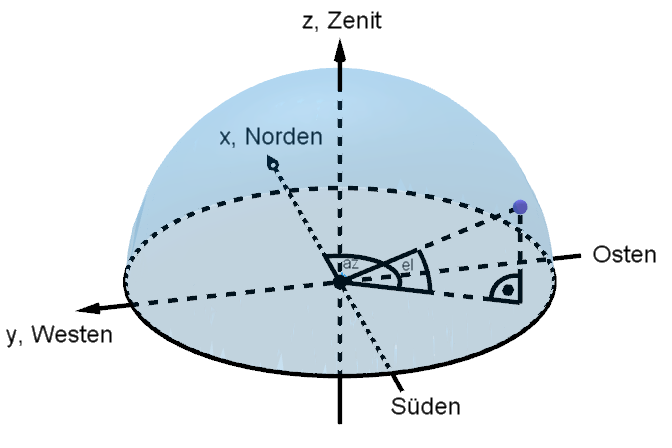
\includegraphics[width=0.7\textwidth]{Images/coordinates.png}
\caption{Die verwendeten Koordinaten}
\label{img:coordinates}
\end{figure}

\section{Entwicklung von Pointingmodellen}
Da man das Teleskop so ausrichten will, das die man die gewünschte Position vorgibt (Koordinaten der CCD- Index C) und dann die Koordinaten am Drive (Index D) einstellt, sucht man nach Funktionen, die die Koordinaten des Drives in Abhängigkeit von den gewünschten Koordinaten beschreibt. 
\begin{equation}
az_D=f_{az}(az_C,el_C)\\
el_D=f_{el}(az_C,el_C)
\label{eq:pointingprinciple}
\end{equation}\\
az_D=f_{az}(az_C,el_C)\\
el_D=f_{el}(az_C,el_C)
\label{eq:pointingprinciple}
\end{equation}\\
Ziel ist es, die Funktionen so zu optimieren, dass die Differenzen zu den gewünschten Koordinaten verschwinden.
\begin{equation}
\Delta{_az}=f_{az}(az_C,el_C)=0\\
\Delta_{el}=f_{el}(az_C,el_C)=0
\label{eq:pointingZero}
\end{equation}\\

\section{Vereinfachtes Pointingmodell mit zwei Parametern}
Zunächst soll ein Pointingmodell mit zwei Parametern entwickelt werden, bei dem die Kamera in der Parkposition ($el_C=0,az_C=0$) in eine andere Richtung zeigt als das Drivesystem ($el_D=el_0,az_D=az_0$). Die beiden Positionen lassen sich auch durch zwei karthesische Richtungsvektoren $\vec{r_D}$ und $\vec{r_C}$ beschrieben. Zunächst wird davon ausgegangen, dass das Teleskop sich in einer Parkposition befindet und anschließend in die gewünschte Position gebracht wird. Als Parkpostion für das Drive-System werden die Koordinaten $el=0$ und $az=0$ gewählt. In karthesischen Koordinaten lässt sich die Richtung durch
\begin{equation}
\vec{r}_D^0=\left(\begin{array}{c} 1 \\ 0 \\ 0 \end{array}\right)
\label{eq:startDrive}
\end{equation}
beschreiben. Durch eine Drehung um die y-Achse mit dem Winkel $el$ und anschließender Drehung die z-Achse um den Winkel $az$ lässt sich aus dieser Startposition jeder Punkt auf der Einheitskugel erreichen. Die beiden Drehungen lassen sich zu einer Transformation $T(az,el)$ zusammenfassen:
\begin{equation}
\nonumber
T(az,el)=R_z(el)R_y(az)=
\left(\begin{array}{ccc} \cos(az) & \sin(el) & 0 \\ -\sin(el) & \cos(el) & 0 \\ 0 & 0 & 1\end{array}\right)
\left(\begin{array}{ccc} \cos(el) & 0 &-\sin(el) \\0 & 1 & 0\\ \sin(el) & 0 & \cos(el) \end{array} \right)
\end{equation}\\
T(az,el)=\left(\begin{array}{ccc} \cos(az)\cos(el) & \sin(az) &-\cos(az)\sin(el) \\-\cos(el)\sin(az) & \cos(az) & \sin(az)\sin(el)\\ \sin(el) & 0 & \cos(el) \end{array} \right)
\label{eq:TransformMat}
\end{equation}\\
Unter der Annahme, dass die Kamera von vornherein in eine andere Richtung als das Drive-System zeigt, lässt sich mit dieser Transformtion $T(az0,el0)$ auch die Startposition der Kamera bestimmen:
\begin{equation}
\vec{r}_C^0=T(az_0,el_0)\vec{r}_D^0=\left(\begin{array}{c} \cos(az_0)\cos(el_0) \\ -\cos(el_0)\sin(az_0) \\ \sin(el_0) \end{array}\right)
\label{eq:startCCD}
\end{equation}
Wendet man nun die gleiche Transformation $T(az_D,el_D)$ auf beide Startvektoren an, so erhält man für jedes Koordinatenpaar des Drives die zugehörigen Koordinaten der CCD in Abhängigkeit der Koordinaten des Drives. Für die Richtung des Drives ergibt sich
\begin{equation}
\vec{r}_D=T(az_D,el_D)\vec{r}_D^0=\left(\begin{array}{c} \cos(az)\cos(el) \\ -\cos(el)\sin(az) \\ \sin(el) \end{array}\right)
\label{eq:finDrive}
\end{equation}
und für die Richtung der CCD
\begin{equation}
\vec{r}_C=T(az,el)\vec{r}_C^0=\left(\begin{array}{c} \cos(az)\left(\cos(az_0)\cos(el)\cos(el_0)-\sin(el)\sin(el_0)\right)-\cos(el_0)\sin(az)\sin(az_0) \\
\sin(az)\left(\sin(el)\sin(el_0)-\cos(az_0)\cos(el)\cos(el_0)\right)-\cos(az)\cos(el_0)\sin(az_0) \\
\cos(az_0)\cos(el_0)\sin(el)+\cos(el)\sin(el_0) \end{array}\right)
\label{eq:finCCD}
\end{equation}
Aus diesen Richtungsvektoren müssen wieder die ursprünglichen Koordinaten $az$ und $el$ rekonstruiert werden. Die Elevation lässt sich aus der z-Komponente (Höhe) berechnen
\begin{equation}
el=\arcsin(r_z)
\label{eq:backtrafoEl}
\end{equation}
und der Azimutwinkel aus dem Verhältnis von y- zu x-Komponente. Allerdings muss man hierbei beachten, in welchem der 4 Quadranten man sich befindet
\begin{equation}
az=\arctan(r_y,r_x)=\left\{\begin{array}{lr}
\arctan\left(\frac{{r_y}}{{r_x}}\right) & r_x \textgreater 0  \\
\arctan\left(\frac{{r_y}}{{r_x}}\right)+\pi &  r_x \textless 0,r_y \textgreater 0 \\
\pm \pi   &  r_x \textless 0,r_y = 0 \\
\arctan\left(\frac{{r_y}}{{r_x}}\right)-\pi &  x \textless 0,r_y \textless 0 \\
+\frac{\pi}{2} &  x = 0,r_y \textgreater 0 \\
-\frac{\pi}{2} & x = 0,r_y \textless 0 \\
\end{array}
\label{eq:backtrafoAz}
\end{equation}

Somit lassen sich mit \ref{eq:backtrafoEl} beziehungsweise mit \ref{eq:backtrafoAz} in Verbindung mit \ref{eq:finCCD} die CCD-Koordinaten in Abhängigkeit der Drive-Koordinaten bestimmen:
\begin{equation}
el_C=\arcsin\left(\cos(az_0)\cos(el_0)\sin(el_D)+\sin(el_0)\cos(el_D)\right)
\label{eq:elD2C}
\end{equation}
\begin{equation}
az_C=\arctan2(x)
\label{eq:azC2D}
\end{equation}
Um die Abhängigkeiten der Drive-Koordinaten von den CCD-Koordinaten zu erhalten, muss das Gleichungssystem \ref{eq:elD2C} \ref{eq:azC2D} nach $el_D$ und $az_D$ aufgelöst werden. Da die Formel \ref{eq:elD2C} nur von $el_D$ und $el_C$ abhängt, kann diese unabhängig von \ref{eq:azC2D} umgestellt werden:
\begin{equation}
el_D=2\arctan\left(\frac{\cos(el_0)\cos(az_0)-\sqrt{\cos^2(el_0)\cos^2(az_0)-\sin^2(el_0)+\sin^2(el_C)}}{\sin(el_C)+\sin(el_0)}
\label{eq:elC2D}
\end{equation}
Stellt man Gleichung \ref{eq:azC2D} nach $az_D$ um, so erhält man
\begin{equation}
az_D=\arctan2\left( x \right)
\label{eq:azC2D}
\end{equation}
wobei hier noch $el_D$ durch den Ausdruck \ref{eq:elC2D} ersetzt werden muss.

\section{Erweiterung des Modells auf vier Parameter}
Einführung additiver Konstanten